%%%%%%%%%%%%% Document Type %%%%%%%%%%%%%
\documentclass[twoside,twocolumn]{article}                          % Article with 2 column
\usepackage[english]{babel}                                         % English document
\usepackage{enumitem}                                               % Items enumeration
\usepackage{array}                                                  % Create tables
\usepackage{eurosym}                                                % € symbol
\usepackage{hyperref}                                               % Internet and pdf links
\usepackage{color}                                                  % Colors for text
\usepackage{fancyhdr}                                               % Type of LaTeX decoration
\usepackage{titlesec}                                               % Style selection
\usepackage{lscape}                                                 % Help top create a large document
\usepackage{amssymb}                                                % Maths symbols
\usepackage[margin=0.8in]{geometry}                                 % Margin
\usepackage{blindtext}                                              % To create blank zones
\usepackage{microtype}                                              % Micro texte
\usepackage[hang, small,labelfont=bf,up,textfont=it,up]{caption}    % Caption modification
\usepackage{lettrine}                                               % First enlarged letter
\usepackage{titlesec}                                               % Allows customization of titles
\usepackage{titling}                                                % Allows customization of title too
\usepackage{authblk}                                                % For multiple authors
\usepackage{graphicx}                                               % Use of graphics and images
\usepackage{etoolbox}                                               % Remove the "References" title of
\patchcmd{\thebibliography}{\section*{\refname}}{}{}{}              % the bibliography


%%%%%%%%%%%%% Configurations %%%%%%%%%%%%%
\linespread{1.05}
\setlist[itemize]{noitemsep}                                        % Make itemize lists more compact
\setlength{\abovecaptionskip}{0pt plus 0pt minus 0pt}               % Change length above caption
\pagestyle{fancy}                                                   % LaTeX style
\fancyhead{}                                                        % Blank out the default header
\fancyfoot{}                                                        % Blank out the default footer
\fancyhead[C]{Improvement of sport by dint of biomimicry - December 2020 - Vol. I, No. 1}% Custom header text

%%%%%%%%%%%%% Title informations %%%%%%%%%%%%%
\setlength{\droptitle}{-4\baselineskip}                             % Move the title up
\pretitle{\begin{center}\Huge\bfseries}                             % Article title formatting
\posttitle{\end{center}}                                            % Article title closing formatting
\title{Improvement of sport by dint of biomimicry}               % Title
\author{LEFAY Paul, CESBRON Théo, HERVE Alexis, GELINEAU Emmanuel, GUYON Soren}                                              % Authors

\renewcommand{\maketitlehookd}{%
\begin{abstract}
  \textbf{Introduction}: This article aims to study several applications of biomimicry to improve human lifestyle. We mostly focus here on the sport field. 
  \textbf{Methods}: First, we looked for general information around biomimicry. Second, we went into more detail around the articles on biomimicry and sport.
  \textbf{Results}: The experiment on swimsuits shows that the one inspired by shark skin generates less hydrodynamic resistance on all drag forces. Also, the use of biomimicry for the knee protector leads to a product more resistant.
  \textbf{Discussion}: Biomimicry is useful and is interesting in a lot of different topics. We show in this article that studying nature and animals can be helpful to improve our skills and capabilities.
  \textbf{Keywords}: Biomimicry, improvement, sports, nature, wildlife, lifestyle.
\end{abstract}
}
\setlength{\columnsep}{25px}                                        % Change the space between 2 columns

%%%%%%%%%%%%% Start of the document %%%%%%%%%%%%%
\begin{document}

%%%%%%%%%%%%% Configurations %%%%%%%%%%%%%
\renewcommand\thesection{\Roman{section}}                           % Roman numerals for the sections
\renewcommand\thesubsection{\roman{subsection}}                     % Roman numerals for subsections

%%%%%%%%%%%%% Header and footer %%%%%%%%%%%%%

\cfoot{\thepage}

\maketitle{}										                                    %Génération du titre

\newpage


\section{Introduction}
\lettrine[nindent=0em,lines=2]{A} s for astronomy or transport, sport is a sector where innovations are numerous. For a longtime, sportsmen and sportswomen tried to achieve better performances by training a lot. The fact is that they finally arrived to the limits of those performances. A way of pushing further those limits is to study new ways of training and additional things to help perform. This article exposes applications of biomimicry : the idea of observing wildlife and transposing its concept in life to solve problems or improve our way of doing things. Through this process, humans managed to make a lot of progress in very varied fields, sport is notably one of them.


\section{Methods}
Biomimicry has a lot of applications in sport and especially in swimming.
In order to improve swimmer’s performances, research led to observation of the fastest fish on Earth and copy it. It appears to be the shark. It has a skin that is so peculiar that water just slides on it and in that way, it allows the shark to have barely no resistance under water. The idea is to recreate the shark’s skin for swimsuits. Experiments were done to find the best material to use and the best way to sew the suit. Both are making great differences for a swimmer in a race. The first experiment was done in a wind tunnel, the study was to understand the aerodynamics of different materials and ways of sewing those materials. The second experiment is based on hydrodynamics. Swimmers are in the pool, they are towed, and with cameras and force data collection, they compare the swim with and without the Fastskin.
de more comfort and flexibility and also keep the same level of protection or even improve it . The design process was completed following the problem driven bio-inspiration approach by working on the armadillo shell\cite{armadillo}.Also, biomimicry has been applied to create better protections for athletes. The idea is to provi

\begin{figure}[!h]
\begin{center}
  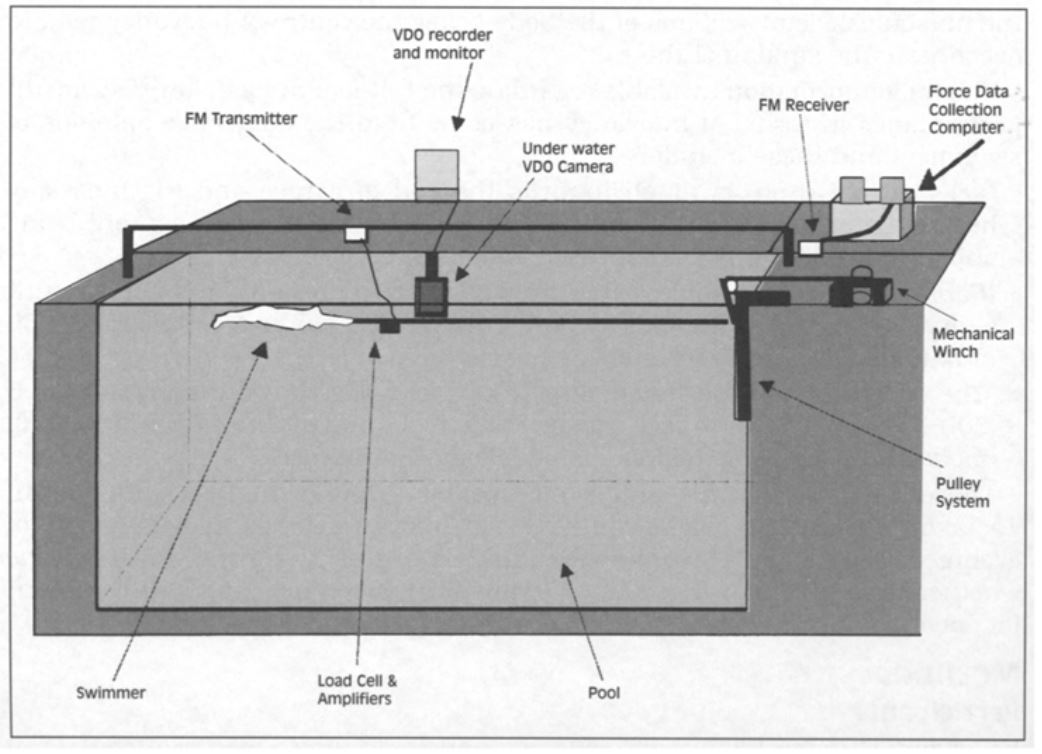
\includegraphics[scale=0.3]{fig2.JPG}
\end{center}
\caption{The towing system and drag recording apparatus}
\end{figure}

\section{Results}
Experiments wich compare standard swimsuits with Fastskin revealed that no denoting differences for hydrostatic weight (p = 0.244) between standard swimsuits and the Fastskin existed. However, figures below provide that the swimsuit inspired by shark skin generated 4.8\% to 10.2\% less hydrodynamic resistance on all drag forces summed together over towing velocities. The aerodynamic experiment shows a drag coefficient value of 0.78 for an usual swimsuit and a value of 0.60 for the Fastskin. 

\begin{center}
\begin{table}[!h]
  \begin{tabular}{ m{35px} m{35px} m{35px} m{35px} m{35px} }
    
    \hline
    Towing Condition & Normal & Fastskin™ & Difference & \% Diff
    \tabularnewline

    \hline
    Surface (gilding) & 347.9 & 328.6 & 19.3 & 5.5
    \tabularnewline

    \hline
    Surface (kicking) & 306.4 & 290.2 & 16.2 & 5.3
    \tabularnewline

    \hline
    Depth (gilding) & 296.9 & 266.7 & 30.2 & 10.2
    \tabularnewline

    \hline
    Depth (kicking) & 282.1 & 268.6 & 13.5 & 4.8
    \tabularnewline

    \hline
    Overall & 1233.3 & 1154.1 & 79.2 & 6.4
    \tabularnewline
    \hline
  \end{tabular}
  \caption{ Drag forces summed over the three towing velocities}
  \vspace{-8mm}
\end{table}
\end{center}

In light of surveys on knee protectors, the armadillo one has to deal with flexibility, comfort, injuries’ protection, an easy installation and an efficient air circulation. Flexibility is based on anthropometric measurements. The new splint is based on the armadillo armour, which structure is made with elastic fiber. The use of biomimicry for the Knee protector leads to a free movements allowed product.
\begin{figure}[!h]
  \begin{center}
    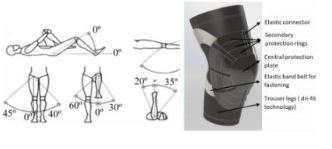
\includegraphics[scale=1.2]{knee2.JPG}
  \end{center}
  \caption{Knee protectors mouvements}
  \end{figure}

\section{Discussion}
Those results mean that biomimicry is used to improve a lot of fields. The Fastskin has less hydrodynamic resistance  which increases the speed of the swimmer by 5\% to 10\%. We found the same progress with the aerodynamic experiment. Results from the survey indicate where are the key points for the specification of the knee protector inspired by armadillo. That leads to focus on flexibility, due to the great mouvement span of the knee and other comfort’s issues such as the air circulation. Those experiments demonstrate that sport’s innovation inspired by animals has gotten better performances or can reach better specification than other technology more easily. By studying nature and animals, we can improve our skills and our capabilities. Such an improvement enables athletes to compete at a higher level as we saw it during the 2004 Olympics where a lot of time records were broken. 

\section{Conclusion}
The initial issue was the fact that we arrived at a point where human performances in sport reach his limit. With the search in the Fastskin, results have been improved. It proves that even if the human body can reach a limit, by working on nature we can improve our capabilities to reach new records. Also, with the example of the knee protectors, we can deduce that biomimicry can be applied to protect the human body. 

\begin{figure}[!h]
  \begin{center}
    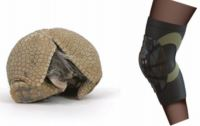
\includegraphics[scale=1]{arma.JPG}
  \end{center}
  \caption{Armadillo knee protectors}
  \end{figure} 

\section{Acknowledgements}
We are grateful to the teams and people who worked on the articles “Comparison of buoyancy, passive and net active drag forces between Fastskin™\cite{Fastskin} and standard swimsuits”, “Contribution of swimsuits to swimmer’s performance”\cite{Swimsuits}, “Bio-Inspired Approach for Innovative Design of Knee Protectors for Recreational Sports”\cite{armadillo}. It enables us to understand how the biomimicry works and was developed through different topics. 






\section{References}
\bibliographystyle{plain}
\bibliography{biblio}

\end{document}